\subsection{Файл с рекордами в игре \q{Block out} и примитивная сериализация}

Многие видеоигры имеют файл с рекордами, иногда называемый \q{Зал славы}.
Древняя игра \q{Block out}\footnote{\url{http://www.bestoldgames.net/eng/old-games/blockout.php}}
(трехмерный тетрис из 1989) не исключение, вот что мы можем увидеть в конце:

\begin{figure}[H]
\centering
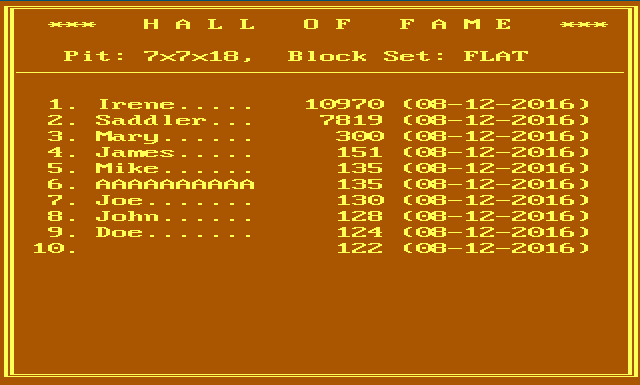
\includegraphics[width=0.7\textwidth]{advanced/550_more_structs/blockout/hs.png}
\caption{Таблица рекордов}
\end{figure}

Мы можем увидеть, что после того как мы добавили свое имя, этот файл изменился: \IT{BLSCORE.DAT}.
Посмотрим на него в Midnight Commander:

\begin{figure}[H]
\centering
\myincludegraphics{advanced/550_more_structs/blockout/mc10.png}
\caption{Файл \IT{BLSCORE.DAT} в Midnight Commander}
\end{figure}

Все записи итак хорошо видны.
Самый первый байт, вероятно, это количество записей.
Второй это 0, и, на самом деле, число записей может быть 16-битным значением, которое простирается на 2 байта.

После имени \q{Irene} мы видим байты 0xDA и 0x2A.
У Irene 10970 очков, и это именно 0x2ADA в шестнадцатеричной системе.
Так что значение рекорда, вероятно, 16-битное целочисленное, а может и 32-битное: после каждого по два нулевых байта.

Подумаем теперь о том факте, что и элементы массива, и элементы структуры всегда располагаются в памяти друг к другу впритык.
\myindex{\CStandardLibrary!write()}
\myindex{\CStandardLibrary!fwrite()}
\myindex{\CStandardLibrary!read()}
\myindex{\CStandardLibrary!fread()}
Это позволяет там записывать весь массив/структуру в файл используя простую ф-цию \IT{write()} или \IT{fwrite()}, 
а затем восстанавливать его используя \IT{read()} или \IT{fread()}, настолько всё просто.
Это то что сейчас называется \IT{сериализацией}.

\subsubsection{Чтение}

Напишем программу на Си для чтения файла рекордов:

\begin{lstlisting}[style=customc]
#include <assert.h>
#include <stdio.h>
#include <stdint.h>
#include <string.h>

struct entry
{
	char name[11]; // включая терминирующий ноль
	uint32_t score;
	char date[11]; // включая терминирующий ноль
} __attribute__ ((aligned (1),packed));

struct highscore_file
{
	uint8_t count;
	uint8_t unknown;
	struct entry entries[10];
} __attribute__ ((aligned (1), packed));

struct highscore_file file;

int main(int argc, char* argv[])
{
	FILE* f=fopen(argv[1], "rb");
	assert (f!=NULL);
	size_t got=fread(&file, 1, sizeof(struct highscore_file), f);
	assert (got==sizeof(struct highscore_file));
	fclose(f);
	for (int i=0; i<file.count; i++)
	{
		printf ("name=%s score=%d date=%s\n",
				file.entries[i].name,
				file.entries[i].score,
				file.entries[i].date);
	};
};
\end{lstlisting}

Нужно добавить атрибут GCC \IT{((aligned (1),packed))}, чтобы все поля структуры были упакованы по 1-байтной границе.

Конечно, это работает:

\begin{lstlisting}
name=Irene..... score=10970 date=08-12-2016
name=Saddler... score=7819 date=08-12-2016
name=Mary...... score=300 date=08-12-2016
name=James..... score=151 date=08-12-2016
name=Mike...... score=135 date=08-12-2016
name=AAAAAAAAAA score=135 date=08-12-2016
name=Joe....... score=130 date=08-12-2016
name=John...... score=128 date=08-12-2016
name=Doe....... score=124 date=08-12-2016
name=Alex...... score=120 date=08-12-2016
\end{lstlisting}

(Нужно добавить, что каждое имя дополнено точками, и на экране, и в файле, вероятно, с эстетическими целями.)

\subsubsection{Запись}

Посмотрим, правы ли мы насчет длины значения очков. Действительно ли там 32 бита?

\begin{lstlisting}[style=customc]
int main(int argc, char* argv[])
{
	FILE* f=fopen(argv[1], "rb");
	assert (f!=NULL);
	size_t got=fread(&file, 1, sizeof(struct highscore_file), f);
	assert (got==sizeof(struct highscore_file));
	fclose(f);

	strcpy (file.entries[1].name, "Mallory...");
	file.entries[1].score=12345678;
	strcpy (file.entries[1].date, "08-12-2016");

	f=fopen(argv[1], "wb");
	assert (f!=NULL);
	got=fwrite(&file, 1, sizeof(struct highscore_file), f);
	assert (got==sizeof(struct highscore_file));
	fclose(f);
};
\end{lstlisting}

Запустим Blockout:

\begin{figure}[H]
\centering
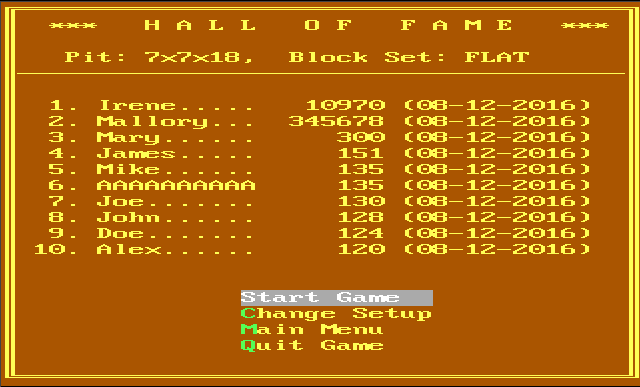
\includegraphics[width=0.7\textwidth]{advanced/550_more_structs/blockout/hs345678.png}
\caption{Таблица рекордов}
\end{figure}

Первые две цифры (1 или 2) пропали. Вероятно, это проблемы с форматированием... но число почти корректно.
Заменяю на 999999 и запускаю снова:

\begin{figure}[H]
\centering
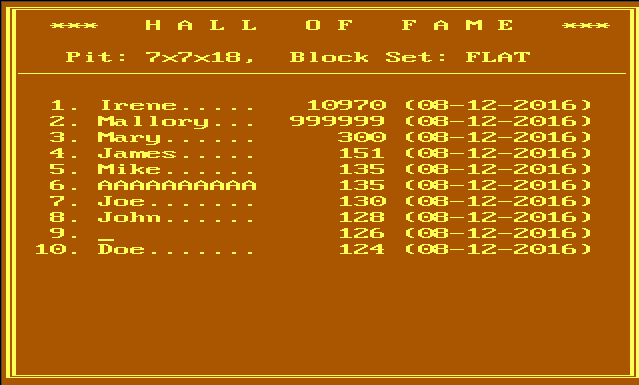
\includegraphics[width=0.7\textwidth]{advanced/550_more_structs/blockout/hs999999.png}
\caption{Таблица рекордов}
\end{figure}

Теперь всё верно. Да, значение очков это 32-битное целочисленное.

\subsubsection{Это сериализация?}

\dots почти.
Сериализация как эта очень популярна в научном и инженерном ПО, где скорость намного важнее чем конвертирование в
\ac{XML} или \ac{JSON} и назад.

Одна очевидная вещь это то что вы, разумеется, не можете сериализировать указатели, потому что каждый раз, когда вы загружаете
файл в память, все структуры могут быть размещены в других местах.

Но: если вы работаете на каком-нибудь маломощном \ac{MCU} с простой \ac{OS} на нем,
и все ваши структуры всегда расположены в тех же местах в памяти, тогда, вы можете сохранять и восстанавливать указатели.

\subsubsection{Случайный шум}

Когда я готовил этот пример, я запускал \q{Block out} много раз и немного играл, чтобы заполнить таблицу рекордов
случайными именами.

И когда было только 3 записи в файле, я увидел это:

\begin{figure}[H]
\centering
\myincludegraphics{advanced/550_more_structs/blockout/mc3.png}
\caption{Файл \IT{BLSCORE.DAT} в Midnight Commander}
\end{figure}

Первый байт это 3, означая, что здесь 3 записи.
И присутствуют 3 записи.
Но затем мы видим случайный шум во второй части файла.

Шум, вероятно, связан с неинициализированными данными.
Вероятно, \q{Block out} выделил память для 10 записей где-то в \glslink{heap}{куче}, где, очевидно, присутствует
некоторый псевдослучайный шум (оставшийся от чего-то еще).
Затем он выставил первый/второй байт, заполнил 3 записи и затем он никогда не трогал оставшиеся 7 записей,
так что они были записаны в файл как есть.

Когда \q{Block out}, при следующем запуске, загружает файл с рекордами, он читает кол-во записей из первого/второго байта (3)
и полностью игнорирует всё, что идет после.

Это распространенная проблема.
Вернее, не совсем проблема в строгом смысле: ничего не глючит, но лишняя информация может попадать наружу.

\myindex{Microsoft Word}
Microsoft Word версий 90-х часто оставлял куски раннее редактированных текстов в файлах *.doc*.
В те времена это было что-то вроде развлечения, получить \IT{.doc}-файл от кого-то, открыть его в шестнадцатеричном редакторе
и прочитать что-то еще, что редактировалось на том компьютере до этого.

\myindex{Heartbleed}
\myindex{OpenSSL}
Эта проблема может быть куда более серьезная: ошибка Heartbleed\footnote{\url{https://en.wikipedia.org/wiki/Heartbleed}}
в OpenSSL.

\subsubsection{Домашнее задание}

\q{Block out} поддерживает несколько поликубов (flat/basic/extended), размер стакана можно конфигурировать, итд.
И похоже на то, что для каждой конфигурации, \q{Block out} имеет свою таблицу рекордов.
Я заметил, что некоторая информация вероятно сохраняется в файле \IT{BLSCORE.IDX}.
Это может быть домашнее задание для хардкорных фанатов \q{Block out} --- разобраться также и в этой структуре.

Файлы \q{Block out} здесь: \url{http://beginners.re/examples/blockout.zip}
(включая двоичные файлы с рекордами, которые я использовал в этом примере).
Для запуска можно использовать DosBox.

